\chapter{建立索引及文献引用}

科研论文或科技报告中的图片、表格、公式和参考文献往往会被编号,方便读者进行查看。在实际写
作过程中,有时图片、表格、公式会不在文本引用位置附近,而参考文献更是一般都总结放在文末结
尾处。因此,读者在阅读过程中,为了查看该处引用内容的详细信息,需要翻看全文查找被引用的内
容。 这个过程一定是非常繁琐低效、并且会影响读者的阅读流畅性。为此,建立索引和文献引用就
非常有必要了。建立索引一般指对文档中的图片、表格、公式等进行索引的设置,这个建立是自动编
号完成;而文献引用同样是对文中存在引用参考文献的地方自动编号建立索引。因此,建立索引和文
献引用的过程较为简单,并且建立索引和引用后的效果非常好,可以实现读者根据索引和文献引用直
接跳转至想要查看的内容,能够有效提高读者的阅读效率和流畅性。

本章节主要包括以下部分:公式和图表的索引、创建超链接并调整链接格式、利用BibTex完成参考
文献引用以及引用格式的设定。

\section{公式和图表的索引}

在第4、5、6、7章中,分别介绍了如何制作或插入公式及图表,在文档中,我们往往需要对公式及图
表进行引用以辅助文档的叙述、描述结果以及佐证一些结论。而有时为了排版的美观,所插入的公式
或图表不一定直接放在引用位置旁边,因此对公式及图表进行索引就显得尤为重要了。

\subsection{公式的索引}

LaTeX中,公式的索引分为主要分为两个部分,一部分是给公式添加标签,可以使用\texttt{\textbackslash{}label\{标签名\}}
命令。根据第4章,可以使用equation环境插入带标签的公式;另一部分是在文档中进行引用,可以
使用\texttt{\textbackslash{}ref\{标签名\}}命令。

\emph{【例】}用label及ref在文中对公式进行索引:
\begin{lstlisting}[language=TeX]
    (\ref{eq1}) is a binary equation

    (\ref{eq2}) is a binary quadratic equation.

    \begin{equation}
    x+y=2\label{eq1}
    \end{equation}

    \begin{equation}
    x^{2}+y^{2}=2\label{eq2}
    \end{equation}
\end{lstlisting}

\subsection{图形的索引}

根据第6章,插入图片需要使用graphicx宏包,图形的索引与公式的索引类似。同样分为两部分,一
部分是使用\texttt{\textbackslash{}label\{标签名\}}命令给添加图形标签,另一部分是使用
\texttt{\textbackslash{}ref\{标签名\}}在文档中进行引用。

\emph{【例】}使用label及ref在文中对图形进行索引:
\begin{lstlisting}[language=TeX]
    \usepackage{graphicx}
    \begin{document}

    Figure \ref{butterfly} is a photo of butterfly.

    \begin{figure}
    \centering
    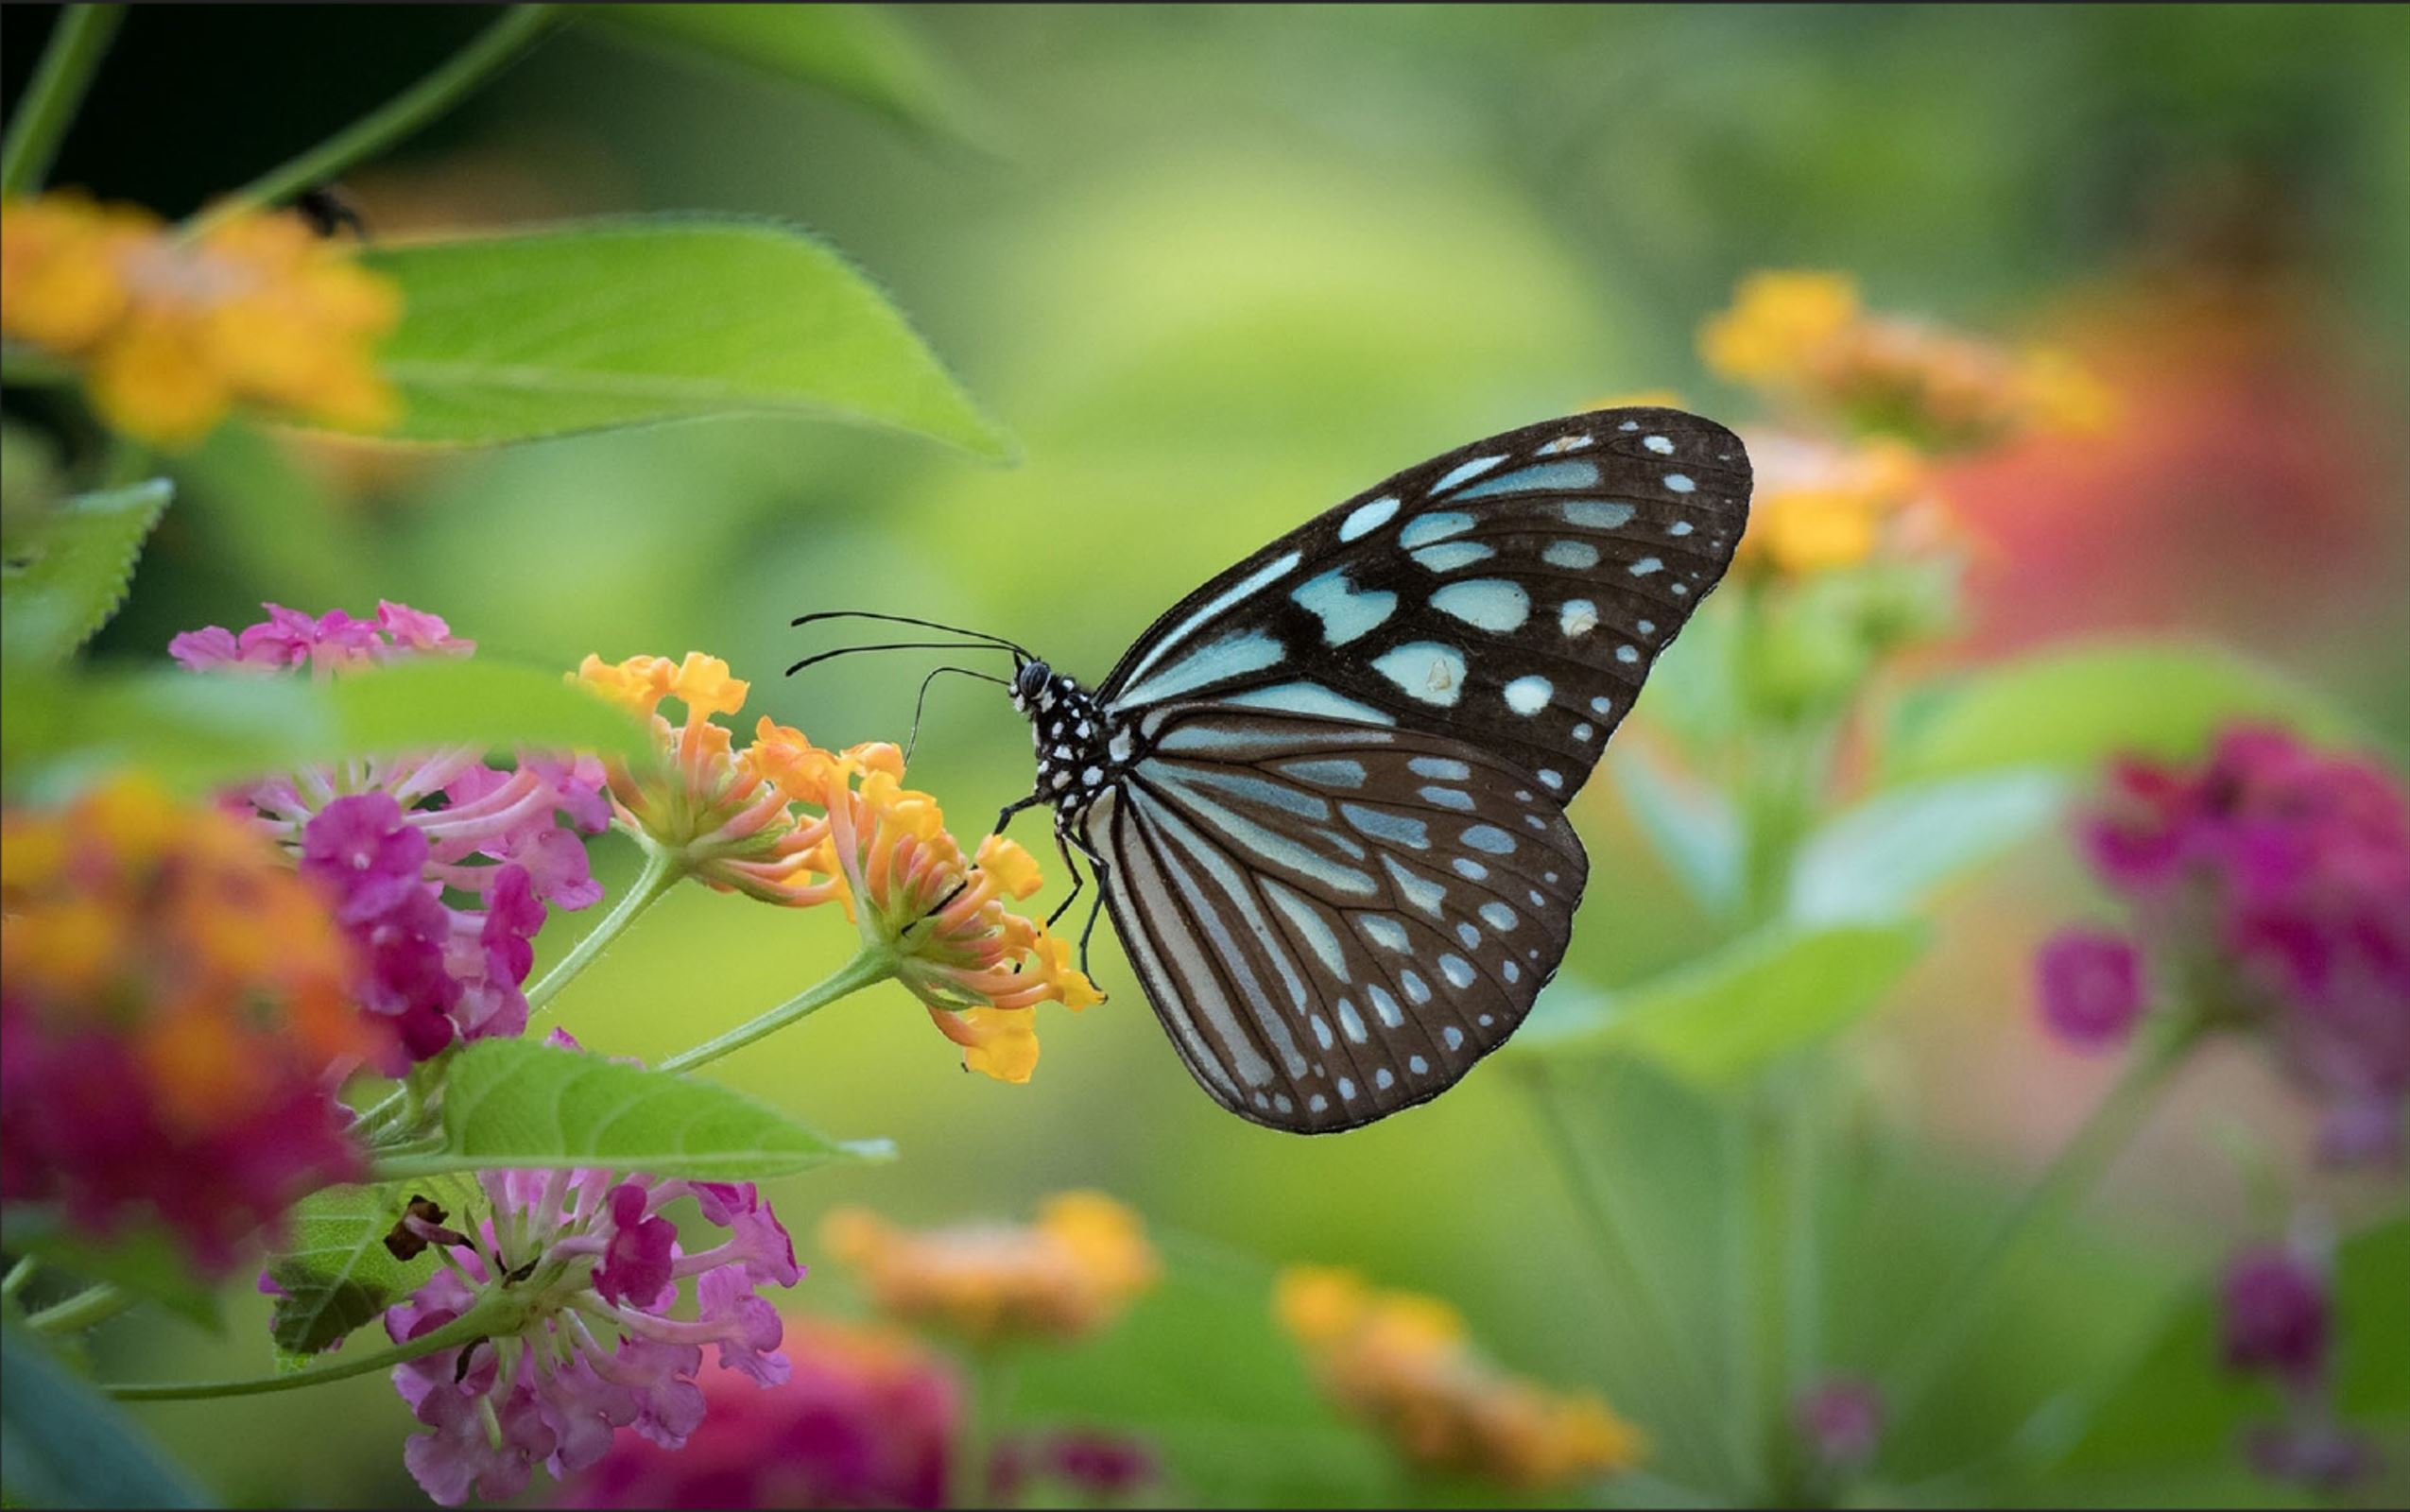
\includegraphics[width = 0.8\textwidth]{graphics/butterfly.JPG}
    \caption{There is a beautiful butterfly.}
    \label{butterfly}
    \end{figure}

    \end{document}
\end{lstlisting}

\subsection{表格的索引}

表格的索引与公式及图形的索引类似,同样分为两部分,一部分是使用\texttt{\textbackslash{}label\{标签名\}}
命令给添加表格标签。根据第5章,可以使用tabular和table两种环境制作带标签的表格;另一部分
是使用\texttt{\textbackslash{}ref\{标签名\}}在文档中进行引用。

\emph{【例】}使用label及ref在文中对图形进行索引:
\begin{lstlisting}[language=TeX]
    Table~\ref{table1} shows the values of some basic functions.

    \begin{table}
        \centering
        \caption{The values of some basic functions.}
        \begin{tabular}{l|cccc}
            \hline
            & $x=1$ & $x=2$ & $x=3$ & $x=4$ \\
            \hline
            $y=x$ & 1 & 2 & 3 & 4 \\
            $y=x^{2}$ & 1 & 4 & 9 & 16 \\
            $y=x^{3}$ & 1 & 8 & 27 & 64 \\
            \hline
        \end{tabular}
        \label{table1}% 索引标签
    \end{table}
\end{lstlisting}

\section{创建超链接}

超链接指按内容链接,可以从一个文本内容指向文本其他内容或其他文件、网址等。超链接可以分为
文本内链接、网页链接以及本地文件链接。LaTeX提供了\emph{hyperref}宏包,可用于生成超链接。
在使用时,只需在前导代码中申明宏包即可,即\texttt{\textbackslash{}usepackage\{hyperref\}}。

\subsection{超链接类型}

\subsubsection{文本内链接}

在篇幅较大的文档中,查阅内容会比较繁琐,因此,往往会在目录中使用超链接来进行文本内容的
快速高效浏览。可以使用hyperref宏包创建文本内超链接。

\emph{【例】}使用label及ref在文中对图形进行索引:
\begin{lstlisting}[language=TeX]
    \documentclass{book}
    \usepackage{blindtext}
    \usepackage{hyperref} %超链接包

    \begin{document}

    \frontmatter
    \tableofcontents
    \clearpage

    \addcontentsline{toc}{chapter}{Foreword}
    {\huge {\bf Foreword}}

    This is foreword.
    \clearpage

    \mainmatter

    \chapter{First Chapter}

    This is chapter 1.


    \clearpage

    \section{First section} \label{second}

    This is section 1.1.
    \end{document}
\end{lstlisting}

在导入\emph{hyperref}时必须非常小心,一般而言,它必须是最后一个要导入的包。

\subsubsection{网址链接}

众所周知,在文档中插入网址之类的文本同样需要用到超链接,同样的,使用hyperref宏包可以创建
网页超链接。有时我们需要将超链接命名并隐藏网址,这时我们可以使用href命令进行插入;有时,
我们插入的网址链接太长,但LaTeX不会自动换行,往往会造成格式混乱的问题,这时,我们可以使用
url工具包,并在该工具包中声明一个参数即可解决这个问题,相关命令为\texttt{\textbackslash{}usepackage[hyphens]\{url\}}。

\emph{【例】}在LaTeX中使用hyperref及url工具包插入网页链接并设置自动换行:
\begin{lstlisting}[language=TeX]
    \usepackage[hyphens]{url}
    \usepackage{hyperref}

    \begin{document}

    This is the website of open-source latex-cookbook repository: \href{https://github.com/xinychen/latex-cookbook}{LaTeX-cookbook} or go to the next url: \url{https://github.com/xinychen/latex-cookbook}.

    \end{document}
\end{lstlisting}

\subsubsection{本地文件链接}

有时,需要将文本与本地文件进行链接,href命令也可用于打开本地文件。

\emph{【例】}在LaTeX中使用href命令打开本地文件:
\begin{lstlisting}[language=TeX]
    \usepackage[hyphens]{url}
    \usepackage{hyperref}

    \begin{document}

    This is the text of open-source latex-cookbook repository: \href{run:./LaTeX-cookbook.dox}{LaTeX-cookbook}.

    \end{document}
\end{lstlisting}

\subsection{超链接格式}

当然,有时候为了突出超链接,也可以在工具包hyperref中设置特定的颜色,设置的命令为\texttt{\textbackslash{}hypersetup},
一般放在前导代码中,例如colorlinks = true, linkcolor=blue, urlcolor = blue, filecolor=magenta。
默认设置以单色样式的空间字体打印链接,\texttt{\textbackslash{}urlstyle\{same\}}命令将
改变这个样式,并以与文本其余部分相同的样式显示链接。

\emph{【例】}在LaTeX中使用hyperref工具包插入超链接并设置超链接颜色为蓝色:
\begin{lstlisting}[language=TeX]
    \usepackage{blindtext}
    \usepackage{hyperref} %超链接包
    \hypersetup{colorlinks = true, %链接将被着色,默认颜色是红色
                linkcolor=blue, % 内部链接显示为蓝色
                urlcolor = cyan, % 网址链接为青色
                filecolor=magenta} % 本地文件链接为洋红色
    \urlstyle{same}

    \begin{document}

    \frontmatter
    \tableofcontents
    \clearpage

    \addcontentsline{toc}{chapter}{Foreword}
    {\huge {\bf Foreword}}

    This is foreword.
    \clearpage

    \mainmatter

    \chapter{First Chapter}

    This is chapter 1.
    \clearpage

    \section{First section} \label{second}

    This is section 1.1.

    This is the website of open-source latex-cookbook repository: \href{https://github.com/xinychen/latex-cookbook}{LaTeX-cookbook} or go to the next url: \url{https://github.com/xinychen/latex-cookbook}.

    This is the text of open-source latex-cookbook repository: \href{run:./LaTeX-cookbook.dox}{LaTeX-cookbook} 

    \end{document}
\end{lstlisting}

\section{BibTeX用法}

LaTeX主要有两种管理参考文献的方法,第一种方法是在\emph{.tex}文档中嵌入参考文献,参考文
献格式需符合特定的文献引用格式;另一种方法则是使用\emph{BibTeX}进行文献管理,文件的拓展
名为\emph{.bib}。其中,使用外部文件BibTeX管理文献更加便捷高效。

\subsection{创建参考文献}

在LaTeX中,插入参考文献的一种直接方式是使用\emph{thebibliography}环境,以列表的形式将
参考文献进行整理起来,配以标签,以供正文引用,文档中引用的命令为\texttt{\textbackslash{}cite\{\}}。

\emph{【例】}使用thebibliography环境在文档中插入参考文献并进行编译:
\begin{lstlisting}[language=TeX]
    Some examples for showing how to use \texttt{thebibliography} environment:
    \begin{itemize}
        \item Book reference sample: The \LaTeX\ companion book \cite{latexcompanion}.
        \item Paper reference sample: On the electrodynamics of moving bodies \cite{einstein}.
        \item Open-source reference sample: Knuth: Computers and Typesetting \cite{knuthwebsite}.
    \end{itemize}

    \begin{thebibliography}{9}
    \bibitem{latexcompanion} 
    Michel Goossens, Frank Mittelbach, and Alexander Samarin. 
    \textit{The \LaTeX\ Companion}. 
    Addison-Wesley, Reading, Massachusetts, 1993.

    \bibitem{einstein} 
    Albert Einstein. 
    \textit{Zur Elektrodynamik bewegter K{\"o}rper}. (German) 
    [\textit{On the electrodynamics of moving bodies}]. 
    Annalen der Physik, 322(10):891–921, 1905.

    \bibitem{knuthwebsite} 
    Knuth: Computers and Typesetting,
    \\\texttt{http://www-cs-faculty.stanford.edu/\~{}uno/abcde.html}
    \end{thebibliography}
\end{lstlisting}

\emph{【例】}使用thebibliography环境在文档中插入参考文献并进行编译:
\begin{lstlisting}[language=TeX]
    \LaTeX{} \cite{lamport94} is a set of macros built atop \TeX{} \cite{texbook}.

    \begin{thebibliography}{9}
    \bibitem{texbook}
    Donald E. Knuth (1986) \emph{The \TeX{} Book}, Addison-Wesley Professional.

    \bibitem{lamport94}
    Leslie Lamport (1994) \emph{\LaTeX: a document preparation system}, Addison
    Wesley, Massachusetts, 2nd ed.
    \end{thebibliography}
\end{lstlisting}

\begin{tcolorbox}[colback=red!5!white, colframe=red!50!black,
        title=参考:]
    https://www.overleaf.com/learn/latex/Bibliography\_management\_with\_bibtex
\end{tcolorbox}

\subsection{使用BibTeX文件}

BibTeX是LaTeX最为常用的一个文献管理工具,它通常以一个独立的文件出现,其拓展名为\emph{.bib}。
它是伴随着LaTeX文档排版系统出现的,1985年兰伯特博士与其合作者开发了这一工具。作为一种特
殊的且独立于LaTeX文件\emph{.tex}之外的数据库,它能大大简化LaTeX文档中的文献引用。实际上,
BibTeX文件中的文献都是用列表的形式罗列的,且不分先后顺序。通过使用引用命令如\texttt{\textbackslash{}cite\{\}}
即可在文档中自动生成特定格式的参考文献,其中,文档中的参考文献格式一般是提前设定好的。

\emph{【例】}使用Bibtex命令一个文献管理文件为sample.bib,将文献按照指定格式进行整理,插入参考文献并进行编译:
\begin{lstlisting}[language=TeX]
    % 创建Bibtex文件,并将其命名为sample.bib

    @article{einstein,
        author =       "Albert Einstein",
        title =        "{Zur Elektrodynamik bewegter K{\"o}rper}. ({German})
            [{On} the electrodynamics of moving bodies]",
        journal =      "Annalen der Physik",
        volume =       "322",
        number =       "10",
        pages =        "891--921",
        year =         "1905",
        DOI =          "http://dx.doi.org/10.1002/andp.19053221004"
    }

    @book{latexcompanion,
        author    = "Michel Goossens and Frank Mittelbach and Alexander Samarin",
        title     = "The \LaTeX\ Companion",
        year      = "1993",
        publisher = "Addison-Wesley",
        address   = "Reading, Massachusetts"
    }

    @misc{knuthwebsite,
        author    = "Donald Knuth",
        title     = "Knuth: Computers and Typesetting",
        url       = "http://www-cs-faculty.stanford.edu/\~{}uno/abcde.html"
    }
\end{lstlisting}

在这三条文献中,einstein、latexcompanion、knuthwebsite是文献的标签,在文档中,只需要
在适当位置用引用命令如\texttt{\textbackslash{}cite\{\}}便可以引用这些文献,例如,\text{\textbackslash{}cite\{einstein\}}。

\begin{lstlisting}[language=TeX]
    Some examples for showing how to use \texttt{thebibliography} environment:
    \begin{itemize}
        \item Book reference sample: The \LaTeX\ companion book \cite{latexcompanion}.
        \item Paper reference sample: On the electrodynamics of moving bodies \cite{einstein}.
        \item Open-source reference sample: Knuth: Computers and Typesetting \cite{knuthwebsite}.
    \end{itemize}

    \bibliographystyle{unsrt}
    \bibliography{sample}
\end{lstlisting}

在sample.bib文件中,根据文献类型可定义文献列表,对于每篇文献,需要整理author(作者信息)、
title(文献标题)等基本信息。在LaTeX文档中,我们需要使用\texttt{\textbackslash{}bibliographystyle}
命令申明参考文献的格式,如本例中的unsrt,同时,使用\texttt{\textbackslash{}ibliography}
命令申明参考文献的源文件,即sample.bib。

当然,BibTeX文献管理也有很多优点:
\begin{itemize}
    \item 无需重复输入每条参考文献。文献放在BibTeX之后,引用文献的标签即可在文档中显示参考文献。
    \item 文档中的参考文献格式是根据文档样式自动设置的,且所有文献的引用风格是一致的。
    \item 引用同一作者同年的文献过多时,引用格式会自动调整。
    \item BibTeX文件中的文献只有在文档中明确引用才会显示在文档的参考文献中。
\end{itemize}

在BibTeX文件中,不同类型的文献是需要进行分类的:
\begin{itemize}
    \item article:对应着期刊或杂志上发表的论文,必须添加的信息有author(作者)、title(标题)、journal(期刊)、year(年份)、volume(卷),可供选择添加的信息包括number(期)、pages(页码)、month(月份)、doi(数字对象识别码)等。
    \item book:对应着书籍,必须添加的信息有author/editor(作者或主编)、title(书名)、publisher(出版社)、year(年份),可供选择添加的信息包括volume/number(卷/期)、series(系列)、address(出版地址)、edition(版号)、month(月份)、url(网址)等。
    \item inbook:书籍中的一部分或者某一章节,必须添加的信息有author/editor、title(标题)、chapter/pages(章节/页码)、publisher(出版社)、year(年份),其他可供选择添加的信息与book一致。
    \item inproceedings:对应着会议论文,必须添加的信息有author(作者)、title(论文标题)、booktitle(论文集标题)、year(年份),可供选择添加的信息包括editor(版号)、volume/number(卷或期)、series(系列)、pages(页码)、address(地址)、month(月份)、organization(组织方)、publisher(出版社)等。
    \item conference:对应着会议论文,与inproceedings用法一致。
    \item mastersthesis和proceedings:分别对应着硕士学位论文和博士学位论文,必须添加的信息有author(作者)、title(标题)、school(学校或研究机构)、year(年份)。
\end{itemize}

\section{文献引用格式}

Bibtex的最大特点是采用了标准化的数据库,对于论文、著作以及其他类型的文献,我们可以自定义
文献的引用格式。Bibtex的样式会改变所引用文献的引用格式。

\subsection{几种标准样式}

一般而言,LaTeX中有一系列标准样式 (standard styles) 可供选择和使用。具体而言,这些标准样式对应的文件包括:
\begin{itemize}
    \item plain.bst
    \item acm.bst:对应于Association for Computing Machinery期刊。
    \item ieeetr.bst:对应于IEEE Transactions期刊。
    \item alpha.bst
    \item abbrv.bst
    \item siam.bst:对应于SIAM。
\end{itemize}

当然,实际上还有很多\emph{.bst}文件,这里给出的几个文件只是最为常用的。不得不提的是\emph{natbib}工具
包,这一工具包对一系列引用命令进行了标准化,而这种标准化不受不同文献样式的影响。

\begin{tcolorbox}[colback=red!5!white, colframe=red!50!black,
        title=Choosing a BibTeX Style:]
    https://www.reed.edu/cis/help/LaTeX/bibtexstyles.html
\end{tcolorbox}